\documentclass[techdoc/techdoc.tex]{subfiles}

\begin{document}

\section{Översikt} \label{sec:3_overview}
Programmet kan delas upp i tre delar: hämtning, bearbetning och inrapportering.
Figur \ref{fig:arch} visar vilka moduler som ingår i varje del och vilken data
som flödar mellan dem.

\begin{figure}[H]
    \centering
    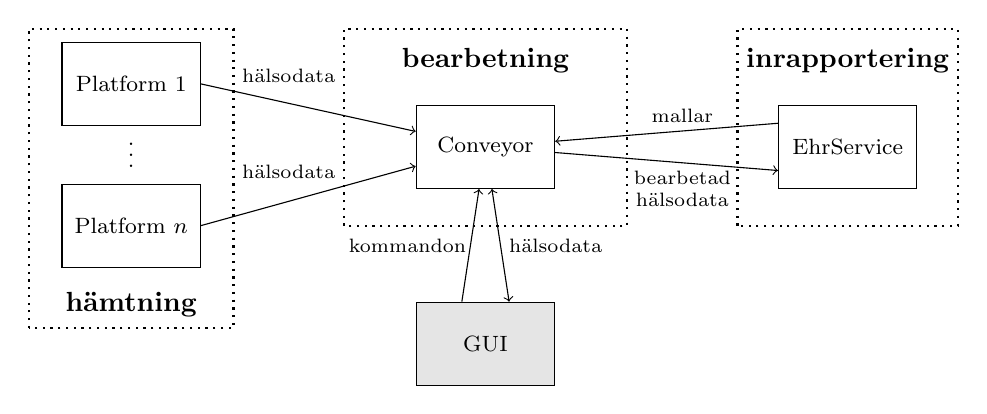
\begin{tikzpicture}[font=\footnotesize]
    \tikzstyle{service}=[rectangle,draw,minimum height=3em,minimum width=5em];
    \tikzstyle{component}=[rectangle,draw,fill=gray!20,minimum height=3em,minimum width=5em];
    \tikzstyle{flow}=[->,font=\scriptsize,text width=2cm,align=center];
    \tikzstyle{group}=[dotted,thick];
    \tikzstyle{grouplabel}=[font=\bfseries];

    \node[service] (plat1) at (-4.5, 0.8) {Platform 1};
    \node[] (platdots) at (-4.5, 0) {$\vdots$};
    \node[service] (platn) at (-4.5, -1) {Platform $n$};

    \node[service] (conv) at (0,0) {Conveyor};
    \node[component] (gui) at (0, -2.5) {GUI};
    \node[service] (ehr) at (4.6, 0) {EhrService};

    \draw[flow] (plat1.east) -- node[above=2mm,xshift=-2.5mm] {hälsodata} (conv);
    \draw[flow] (platn.east) -- node[above=1mm,xshift=-2.5mm] {hälsodata} (conv);

    \draw[flow] ([xshift=-3mm]gui.north) -- node[xshift=-8mm] {kommandon} (conv);
    \draw[flow,<->] (conv) -- node[xshift=7mm] {hälsodata} ([xshift=3mm]gui.north);

    \draw[flow] ([yshift=3mm]ehr.west) -- node[above,xshift=2mm] {mallar} (conv);
    \draw[flow] (conv) -- node[below,xshift=2mm] {bearbetad hälsodata} ([yshift=-3mm]ehr.west);

    \draw[group] (-5.8,-2.3) rectangle (-3.2, 1.5);
    \draw[group] (-1.8,-1) rectangle (1.8, 1.5);
    \draw[group] (3.2,-1) rectangle (6, 1.5);

    \node[grouplabel] at (-4.5,-2) {hämtning};
    \node[grouplabel] at (0,1.1) {bearbetning};
    \node[grouplabel] at (4.6,1.1) {inrapportering};
\end{tikzpicture}

    \caption[Översiktlig programarkitektur]{Översiktliga delar och dataflödet
    mellan dem.}
    \label{fig:arch}
\end{figure}

Alla händelser styrs utifrån kommandon från det grafiska gränssnittet i
GUI-modulen. GUI-modulen kommunicerar endast med Conveyor, som fungerar som en
fasad, vilket innebär att arkitekturen till viss grad följer ett fasadmönster.
Fasaden ser efter vilka datakategorier och plattformar som finns tillgängliga.

\subsection{Programflöde}
Vid ett typiskt programflöde frågar GUI-modulen fasaden först vad det finns för
plattformar att hämta data ifrån. Därefter väljer GUI-modulen en plattform och
frågar fasaden vilka kategorier av hälsodata som finns tillgängliga för den
plattformen. Fasaden får en lista av mallar för kategorier från EhrService.
Fasaden kollar därefter vilka av dessa mallar som stöds av den valda
plattformen och returnerar dem för utskrivning i GUI:et.

GUI-modulen väljer därefter en kategori och ber fasaden att hämta datan. Då
anropas implementationen för plattformen och datan lagras i fasaden. Därefter
kan GUI-modulen hämta och modifiera datan i fasaden för uppvisning och
komplettering från användaren. När användaren har bearbetat och granskat
hälsodatan ber GUI-modulen fasaden att skicka upp datan vilken i sin tur låter
EhrService skicka datan till patientens journal.

\subsection{Moduler och filstruktur}
Den övergripande filstrukturen kan ses i figur \ref{fig:files}. Applikationen
följer huvudsakligen Angulars filstruktur som beskrivet i sektion \ref{sec:ng}.

\begin{figure}[H]
    \lstinputlisting{techdoc/lst/file_structure}
    \caption{Övergripande filstruktur av applikationens källkod.}
    \label{fig:files}
\end{figure}

Utöver det har programmets filer delats upp i tre delar: \texttt{platform},
\texttt{gui} och \texttt{ehr}. Hämtningen av hälsodata hanteras i
\texttt{platform}, som innehåller en superklass \texttt{Platform} samt en
specifik underklass för varje plattform såsom \texttt{GfitService}.
Inrapporteringen av hälsodata och hanteringen av all kommunikation mot RÖD
sköts i \texttt{ehr}, som även innehåller de datastrukturer som är baserade på
openEHR. Till sist återfinns applikationens grafiska komponenter i
\texttt{gui}.

\texttt{app} innehåller även en mapp \texttt{shared} som i sin tur innehåller
filer som ej är bundna till en specifik modul, exempelvis en klass som
specificerar en tidsperiod.

\end{document}
